\section{Evaluation}\label{s:eval}

%We have seen in Figure~\ref{fig:design:shift-bottleneck} that \name can move the network queues to the \inbox to gain control over scheduling. 
%Given that this is possible, what benefits can \name achieve, and where do they come from?
Given \name's ability to move the in-network queues to the \inbox (as shown earlier in Figure~\ref{fig:design:shift-bottleneck}), we now explore:
\begin{enumerate}[leftmargin=15pt]
    \item Where do \name's performance benefits come from? We discuss this in the context of improving the flow completion times of \name's component flows. (\S\ref{s:eval:fct})
    \item Can \name enforce different scheduling policies? (\S\ref{s:eval:policies})
    \item Do \name's performance benefits hold across different scenarios? (\S\ref{s:robust:cross})
    %\item Under what conditions do \name's performance benefits hold? (\S\ref{s:robust:cross})
\end{enumerate}
\fc{Come back and update these after eval is finished}


\subsection{Experimental Setup}\label{s:eval:setup}

We evaluate our implementation of \name (discussed in \S\ref{s:impl}) using network emulation via mahimahi~\cite{mahimahi}.
Mahimahi creates a Linux network namespace and applies the configured network condition (emulated delay or link bandwidth) to all packets that traverse it. 

There are three $8$-core machines in our setup: one machine is a sender, another is configured as a middlebox and runs a \inbox, and a third is the receiver. The \outbox runs on the same machine as the receiver, inside the same mahimahi network namespace as the receiving application. 
Our prototype requires that the sending application and the \inbox run on different machines, to prevent TCP small queues (TSQ) from interfering with the queuing behaviour that one would expect in a real deployment. 
%It is important for experiment fidelity to run the sending application on a different machine than the \inbox; otherwise, because the \inbox data-path uses tc (\S\ref{s:impl}), TCP small queues (TSQ) unrealistically avoids queueing.
Since our \outbox implementation uses \texttt{libpcap}, GRO would change the packets before they are delivered to the \outbox, which would cause inconsistent epoch boundary identification between the two boxes. We, therefore, disable TSO and GRO.
Throughout our experiments, CPU utilization on the machines remained below $10$\%.

% \an{somebody make sure this makes sense}\an{Since our prototype implementation uses the Linux kernel datapath, we disable TCP segmentation offload (TSO) and generic receive offload (GRO) on the machines to maintain a consistent view of packet headers between the \inbox and the \outbox.
% This is an artifact of our prototype implementation of the \outbox using \texttt{libpcap}: in a real deployment, the \outbox would have the same view of the packets as the \inbox.}
Unless otherwise specified, we emulate the following scenario.
A many-threaded client generates requests from a request size CDF drawn from an Internet core router~\cite{caida-dataset}, and assigns them to one of $200$ server processes on the traffic generator.
The workload is heavy-tailed: 97.6\% of requests are 10KB or shorter, and the largest 0.002\% of requests are between $5$MB and $100$MB.
Each server then sends the requested amount of data to the client and we measure the flow completion time of each such request. 
%\an{In addition, the server also generates a persistently backlogged connection to the client.}
%We use multiple server processes to emulate multiple machines behind the \name at the customer's edge.
The link bandwidth at the mahimahi link is set to 96Mbps, and the RTT is set to 50ms. The requests result in an offered load of 84Mbps. 

The endhost runs Cubic~\cite{cubic} congestion controller, and the \inbox runs Copa~\cite{copa} (we test other schemes in \S\ref{s:eval:cc}) with the Nimbus~\cite{nimbus} elasticity detection mechanism. The \inbox schedules traffic using stochastic fair queueing~\cite{sfq} in our experiments by default (we use other policies in \S\ref{s:eval:policies}). Each experiment is comprised of $100,000$ requests sampled from this distribution, across $10$ runs each with a different random seed. 

\subsection{Understanding Performance Benefits}\label{s:eval:fct}

We first present results for a simplified scenario without any cross-traffic, i.e. all traffic traversing through the network is generated by the same customer and is, therefore, part of the same bundle. 
This scenario highlights the benefits of using \name when the congestion on the bottleneck link in the network is self-inflicted. We explore the effects of congestion due to other cross-traffic in \S\ref{s:robust:cross}.

%that models a background large data transfer which would normally fill the bottleneck queue.
%
%\radhika{another title for this section, or some preceding explanation on what each section is about}
%
%\cut{Note that it is important to use many server processes so that the effect of head-of-line blocking on the client requests is limited.
%Indeed, all the CDFs presented in this section have a ``knee'' where the effects of head-of-line blocking become apparent.
%}
%\radhika{when the graphs are presented, explain the `knee' as an artifact of our expts caused due to some HoL blocking. Btw, are you sure that's why you have the knee?}

\begin{figure}
    \centering
\begin{knitrout}
\definecolor{shadecolor}{rgb}{0.969, 0.969, 0.969}\color{fgcolor}
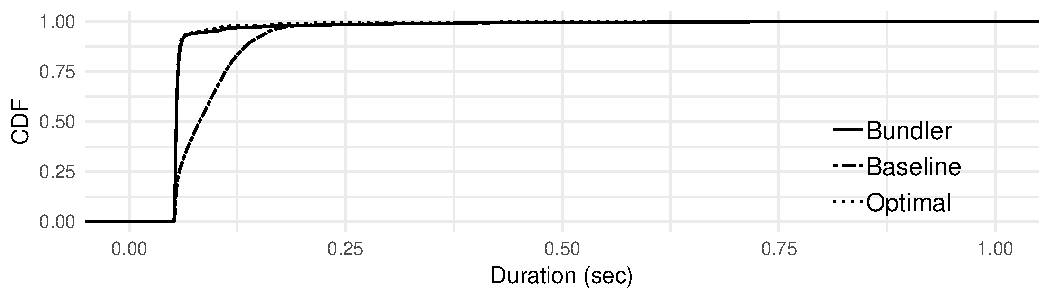
\includegraphics[width=\maxwidth]{figure/eval:best-1} 

\end{knitrout}
    \caption{\name achieves $33$\% lower median slowdown. Note the differing axis scales. For both \name and Optimal, performance benefits come from preventing short flows from queueing behind long ones. \an{Whiskers currently show 1.25 inter-quantile range, figure out how to show 99th \%ile? Also, can barely see Bundler and Optimal...}}
    \label{fig:eval:best}
\end{figure}

\newcommand{\baseline}{Status Quo\xspace}
\newcommand{\optimal}{In-Network\xspace}

%\paragrapha{Comparison with \baseline and \optimal Scheduling} 
\Para{Using \name for fair queueing}
%On a $96$Mbps link, we generate  from the CDF described above.
In this section, we evaluate the benefits provided by doing fair queuing at the \name, and use median slowdown as our metric, where the ``slowdown'' of a request as its completion time divided by what its completion time would have been in an unloaded network. A slowdown of $1$ is optimal, and lower numbers represent better performance.

We evaluate three configurations: 
(i) The ``\baseline'' configuration represents the status quo: the \inbox simply forwards packets as it receives them, and the mahimahi bottleneck uses FIFO scheduling.
(ii) The ``\optimal'' configuration deploys fair queueing\footnote{
We implement this scheme by modifying mahimahi (our patch comprises $171$ lines of C++) to add a packet-level fair-queueing scheduler to the bottleneck link.}
at the mahimahi bottleneck. 
Recall from \S\ref{s:intro} that this configuration is not enforced in practice.
%: it would force all customers --- who may desire diverging scheduling policies --- to use the same scheduler.
(iii) The default \name configuration, that uses stochastic fair queueing~\cite{sfq} scheduling policy at the \inbox.
%(iv) Finally, perform a factor analysis for \name, we also evaluate a configuration where \name does FIFO scheduling. 


Figure~\ref{fig:eval:best} presents our results. 
As is expected from the use of fair queuing, \name is able to achieve significant reductions in the slowdown for short flows, followed by some reduction for medium-sized flows, and similar performance for large flows. 
%\name, using fair queueing, significantly improves the slowdown for short ($<$10KB) flows, while the medium
The median slowdown
%\footnote{We define the ``slowdown'' of a request as its completion time divided by what its completion time would have been in an unloaded network. A slowdown of $1$ is optimal, and lower numbers represent better performance.} 
decreases from \overviewBenefitsBaselineMedian 
for Baseline to \overviewBenefitsBundlerMedian 
with \name: \overviewBenefitsBundlerMedianImprovement
lower. 
%Note that the corresponding reductions in median flow completion time is also \overviewBenefitsBundlerMedianImprovement. 

Furthermore, \name's performance is close to \optimal.
Both \name and \optimal achieve an identical median slowdown of \overviewBenefitsBundlerMedian.
\optimal provides better performance in the tail: the $99\%$ile slowdown is \overviewBenefitsOptimalTail for ``\optimal'' and \overviewBenefitsBundlerTail for \name.
Meanwhile, the \baseline achieves a $99\%$ile slowdown of \overviewBenefitsBaselineTail.
%We next discuss the source of this higher tail FCT compared to \optimal.

\paragrapha{FIFO is not enough} It is important to note that \name by itself (i.e. running FIFO scheduling) is not a means of achieving improved performance. 
%as promised by recent efforts in congestion control~\cite{copa, nimbus}, 
despite doing aggregated congestion control across all flows in a bundle.
To see why this is the case, recall that \name does not modify the endhosts: they continue to run the default Cubic congestion controller, which will probe for bandwidth until it observes loss.
Indeed, the packets endhost Cubic sends beyond those that the link can transmit must be queued somewhere in the network or get dropped. Without \name, they get queued up at the bottleneck link. With \name, they instead just get queued up at the \inbox. In addition, the congestion controller at \inbox also maintains a small standing queue at the bottleneck link (which can be seen in Figure~\ref{fig:design:shift-bottleneck}) to avoid under-utilization, which increases the end-to-end-delays slightly. Therefore, doing the FIFO scheduling at the \name, as is done by the \baseline, results in slightly worse performance (shown in Figure~\ref{fig:eval:fifo}).
%As a result, \emph{solely} using a more sophisticated congestion control algorithm at the \name is unlikely to be the cause of significant reductions in the flow completion time.

\begin{figure}
    \centering
\begin{knitrout}
\definecolor{shadecolor}{rgb}{0.969, 0.969, 0.969}\color{fgcolor}
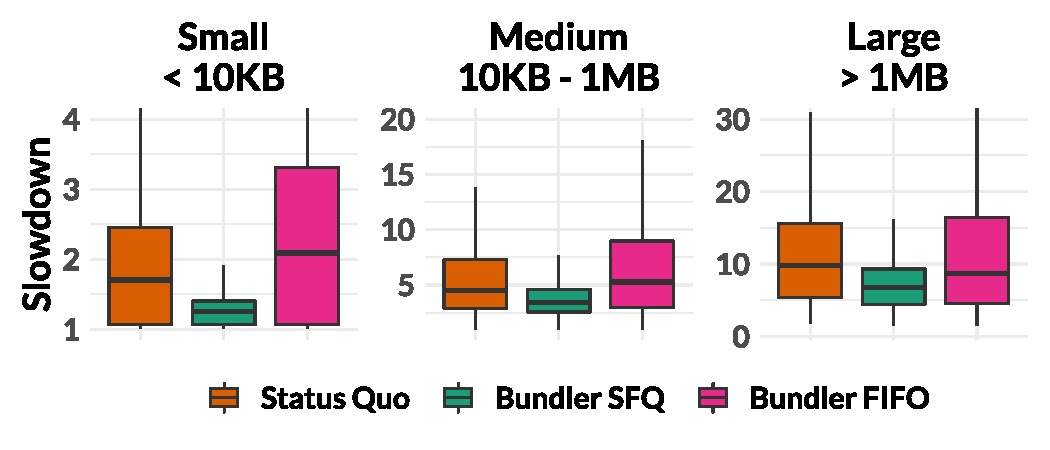
\includegraphics[width=\maxwidth]{figure/eval_fifo-1} 

\end{knitrout}
    \caption{With FIFO scheduling, the benefits of \name are lost: FCTs are 31\% worse in the median. Note the different y-axis scales for each group of request sizes.}
    \label{fig:eval:fifo}
\end{figure}
\newcommand{\overviewBenefitsFifoMedian}{2.13\xspace}
\newcommand{\overviewBenefitsFifoWorse}{31\%\xspace}

% This is why the tail FCT for \name does not match \optimal's.
% We can see this by measuring the relative performance of using FIFO scheduling at the \name instead of the SFQ scheduling in Figure~\ref{fig:eval:best}.
% The results are in Figure~\ref{fig:eval:fifo}. 
% Unsurprisingly, the FCTs with FIFO scheduling at \name are \emph{worse}: with a median slowdown of \overviewBenefitsFifoMedian, it is \overviewBenefitsFifoWorse higher than the \baseline. 

\subsection{Real Internet Paths}\label{s:eval:realworld}
\begin{figure}
    \centering
\begin{knitrout}
\definecolor{shadecolor}{rgb}{0.969, 0.969, 0.969}\color{fgcolor}
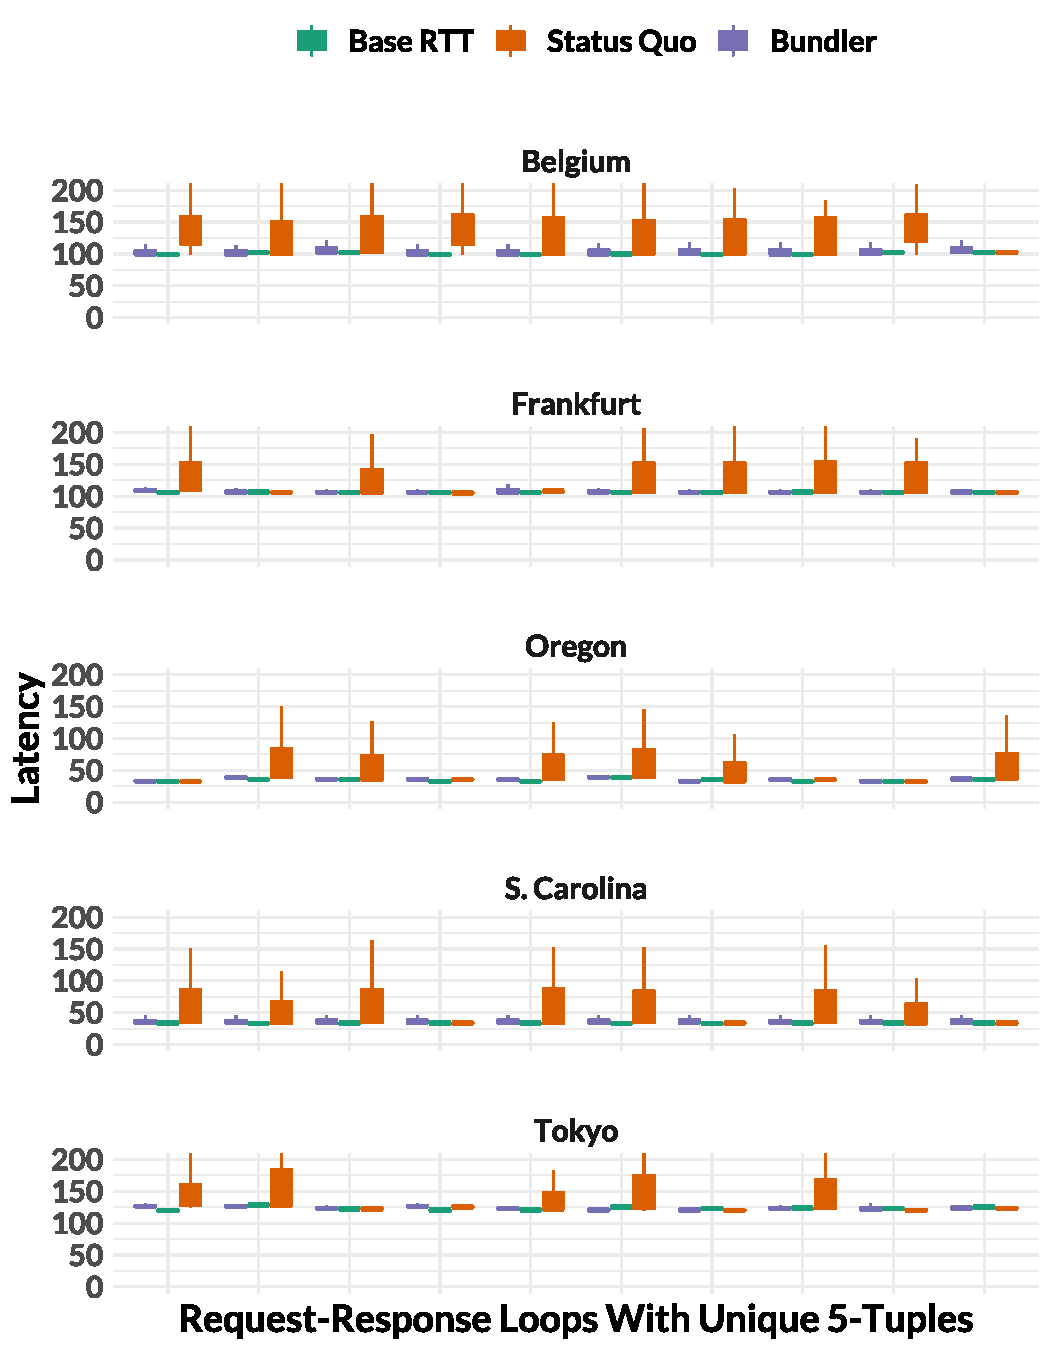
\includegraphics[width=\maxwidth]{figure/eval:realworld-1} 

\end{knitrout}
    \caption{On 5 real-Internet paths from the GCP datacenter in Iowa, \name achieves close to the Base RTT for latency-sensitive traffic. Each bar depicts an individual 5-tuple. On some paths, load-balancing in the Internet causes only some 5-tuples to experience queueing. \name offers scheduling for those paths.}
    \label{fig:eval:realworld}
\end{figure}
%\newcommand{\overviewBenefitsBundlerMedianImprovement}{round(100*(1-(overview_benefits_bundler_results[1] / overview_benefits_baseline_results[1])), 0)\%\xspace}

Is there queueing on real Internet paths, and if so, can \name effectively control those queues?
An interesting real-Internet scenario to consider is load-balancing, a widely used technique for reducing the congestion on any one path.
Here, we make two observations: 
(1) while bundle traffic may traverse multiple intermediate paths, it will converge on the receiving domain (and the \outbox). If the bottleneck is near the receiving domain, the bundled traffic will still build queues.
(2) from the bundle's perspective, multiple paths appear as multiple queues, with some aggregate bandwidth capacity (\ie the max-flow of the network paths between the sending and receiving domains). While queueing may be unevenly distributed among the paths, the distribution of flows onto paths is currently random (\eg via ECMP). With \name, all these queues are moved to the \inbox, so it can schedule bundled flows deliberately rather than randomly.

To measure this effect, we measure the latency of 10 parallel, closed-loop UDP senders with 40-byte requests. Each UDP sender uses a different port, to gain visibility across multiple paths, if applicable.
We gather baseline latency measurements on five bundles sent from a GCP datacenter in Iowa to GCP datacenters in Belgium, Frankfurt, Oregon, South Carolina, and Tokyo and measure queueing\footnote{We use GCP's ``Standard Networking'' option, since our focus is the public Internet.}
by comparing this baseline to the same scenario with 20 backlogged senders.
Figure~\ref{fig:eval:realworld} shows one set of box-plots for each 5-tuple, for each of the five bundles. ``Base RTT'' bars show the latency without backlogged senders and ``Status Quo'' bars represent, as above, the latency with the backlogged senders but without \name.
We observe multipath effects for all five bundles; while, as a result, some paths experience no queueing, all five bundles also experience queueing on at least half of the available paths.

On the paths with queueing, becase \name can prioritize the latency-sensitive requests, the latency those requests observe is significantly reduced. As a result, across the bundle as a whole, \name achieves \realworldMedianLatencyImprovement lower latencies than the status quo scenario over the 5 paths.

\subsection{Applying Different Scheduling Policies}\label{s:eval:policies}
%Per \S\ref{s:impl}, our \name implementation can implement any scheduling discipline available in Linux. 
We demonstrate that, in addition to improving flow completion times, our implementation of \name can achieve low packet delay, perform strict prioritization, and rate fairness.

\paragrapha{Achieving Improved Flow Completion Times} \S\ref{s:eval:fct} shows how enabling SFQ at the \name improves the median slowdown by \overviewBenefitsBundlerMedianImprovement.

\paragrapha{Achieving Low Packet Delays}
We enable CoDel~\cite{fq-codel} at the \inbox, to lower the packet delays, and test it for a single large backlogged flow, using the setup described in \S\ref{s:eval}.
%, which adds ECN marks to packets in fair-queue buckets which exceed a threshold. 
%As a result, endhosts cut their windows earlier than otherwise, and thus achieve low end-to-end-delays.
We measure the distribution of RTTs seen by the endhost connections with \name and \baseline.
\begin{figure}
    \centering
\begin{knitrout}
\definecolor{shadecolor}{rgb}{0.969, 0.969, 0.969}\color{fgcolor}
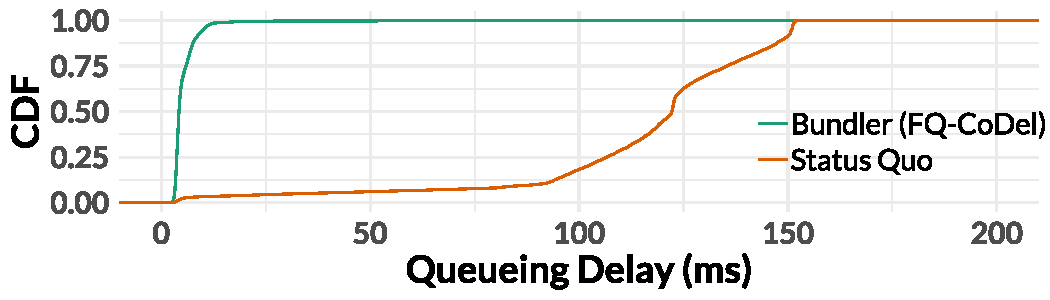
\includegraphics[width=\maxwidth]{figure/eval:lowdelays-1} 

\end{knitrout}
    \caption{We configure \name with the fq-codel scheduling policy to achieve low end-to-end queueing delays.}
    \label{fig:eval:lowdelays}
\end{figure}

As is expected from CoDel, \name in this experiment, achieves \delaysImprovement lower median packet delay than \baseline.
%Note that due to the effect discussed above, using FIFO scheduling results in higher delays than the \baseline case.

\paragrapha{Strict Prioritization}\label{s:eval:strictprio}
We uniformly divide the web request distribution described in \S\ref{s:eval:setup} into two classes, one of which is given a higher priority over the other. The results are presented below.
%of traffic transitting \name over a lower-priority class. 

\begin{table}[h]
\begin{center}
\begin{tabular}{c|c|c}
Scheme     &  Median Slowdown                           &  $99$\%ile Slowdown                        \\
\hline
Bundler (Prio.)   &  1.07 &  10.52  \\
Bundler (SFQ)     &  \overviewBenefitsBundlerMedian  &  \overviewBenefitsBundlerTail  \\
\baseline  &  3.07  &  201.72
    \label{fig:eval:strict-prio}
\end{tabular}
\end{center}
\caption{Using strict prioritization further reduces FCTs for the higher-priority class of traffic.}\label{t:eval:prio}
\end{table}
\newcommand{\strictPrioTailImprovementOverFq}{47\%\xspace}
\newcommand{\strictPrioImprovement}{65\%\xspace}


Using a priority scheduler at \inbox improves the flow completion times for the higher-priority class when compared to \baseline.
Furthermore, prioritization achieves \strictPrioTailImprovementOverFq lower $99$\%ile FCT for the higher priority traffic class, when compared to using fair queueing instead.
%running this scenario with to fair queueing,.

\begin{figure}
    \centering
\begin{knitrout}
\definecolor{shadecolor}{rgb}{0.969, 0.969, 0.969}\color{fgcolor}
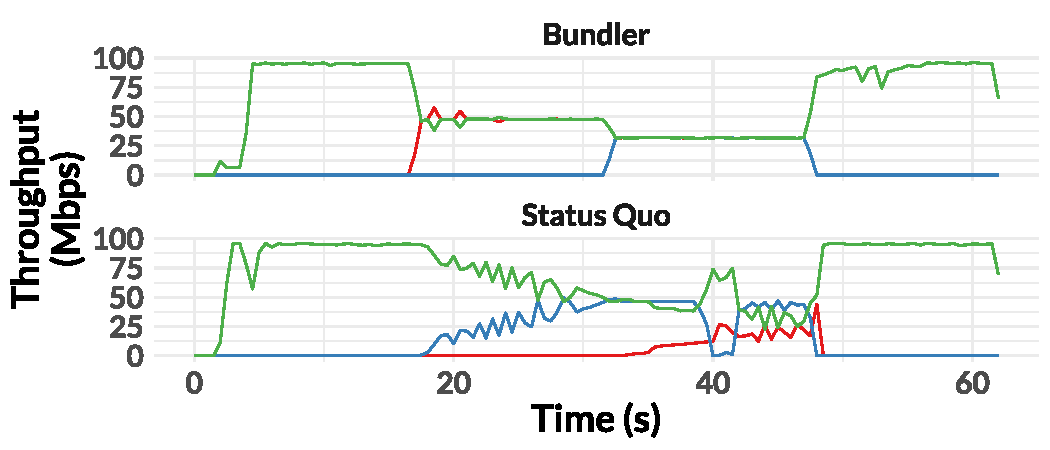
\includegraphics[width=\maxwidth]{figure/eval_waterfall-1} 

\end{knitrout}
    \caption{\name with SFQ achieves fair and stable rates.}
    \label{fig:eval:waterfall}
\end{figure}

\paragrapha{Rate Fairness and Stability}\label{s:eval:waterfall}
We next use our default SFQ scheduler to achieve fairness and rate stability. We start three backlogged flows at different times (0s, 15s, and 30s). Figure~\ref{fig:eval:waterfall} shows that \name converges to fair and stable rates faster than the \baseline.

\cut{
\begin{figure}
    \label{fig:eval:video}
    \centering
    \begin{subfigure}[b]{0.5\textwidth}
        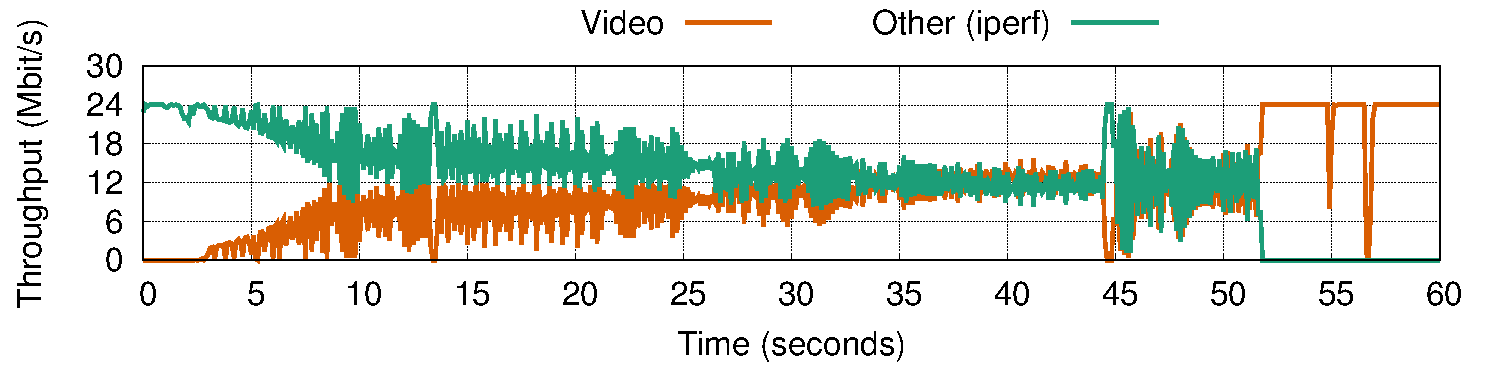
\includegraphics[width=\textwidth]{figure/nobundle-4k-video}
        \caption{Without \name}\label{fig:eval:video:nobundle}
    \end{subfigure}
    \begin{subfigure}[b]{0.5\textwidth}
        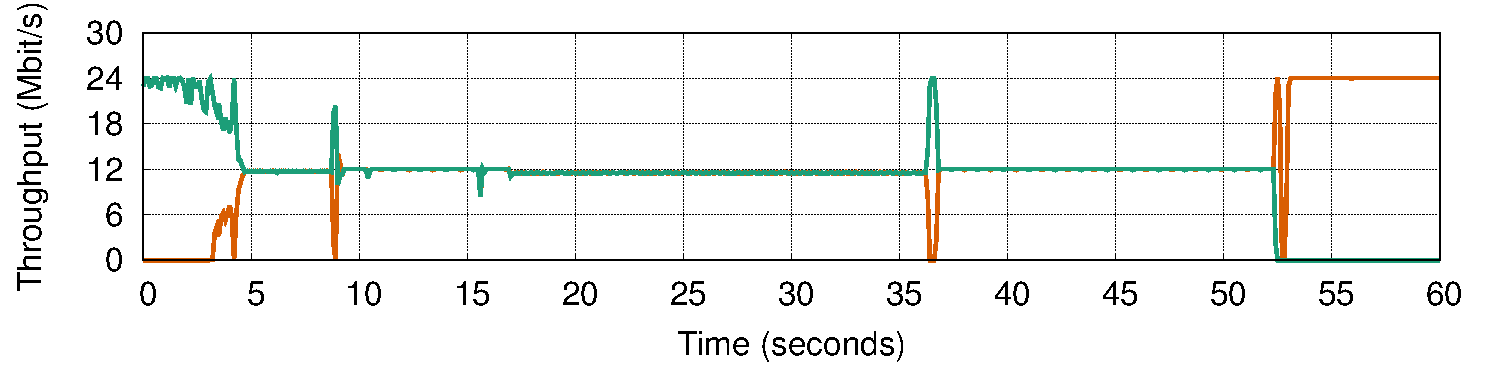
\includegraphics[width=\textwidth]{figure/bundle-4k-video}
        \caption{With \name}\label{fig:eval:video:bundle}
    \end{subfigure}
    \caption{Without \name, the video traffic experiences highly variable throughput, which prevents the ABR algorithm from realizing it could sustain a higher bitrate. \name helps the video flow to quickly converge to the fair rate and stay there, which allows the ABR algorithm to choose the maximum sustainable bitrate.}
\end{figure}

\paragrapha{Rate Stability}\label{s:eval:ratestable}
\fc{come back to this}
In Figure~\ref{fig:eval:video}, we run a persistently backlogged flow over a 24Mbps link and then
after 3 seconds start a client attempting to stream a 4k video from a server that supports adaptive
bitrate selection. Without \name (a), the video stream experiences highly variable throughput and 
takes 30 seconds to converge to a fair share of the link. In contrast, with \name (b), the video
stream converges to its fair share within 2 seconds and is able to maintain that rate for the
entirety of the stream. This stability provides the best scenario for the ABR algorithm to select
the highest possible bitrate and thus maximize QoE.
}


\subsection{Impact of Cross Traffic}\label{s:robust:cross}


\newcommand{\bigexpBundlerElasticSlowdown}{2.6251566\%\xspace}
\newcommand{\bigexpNoBundlerElasticSlowdown}{2.3453956\%\xspace}
\newcommand{\bigexpElasticSlowdownWorseness}{12\%\xspace}

\begin{figure*}
\begin{centering}
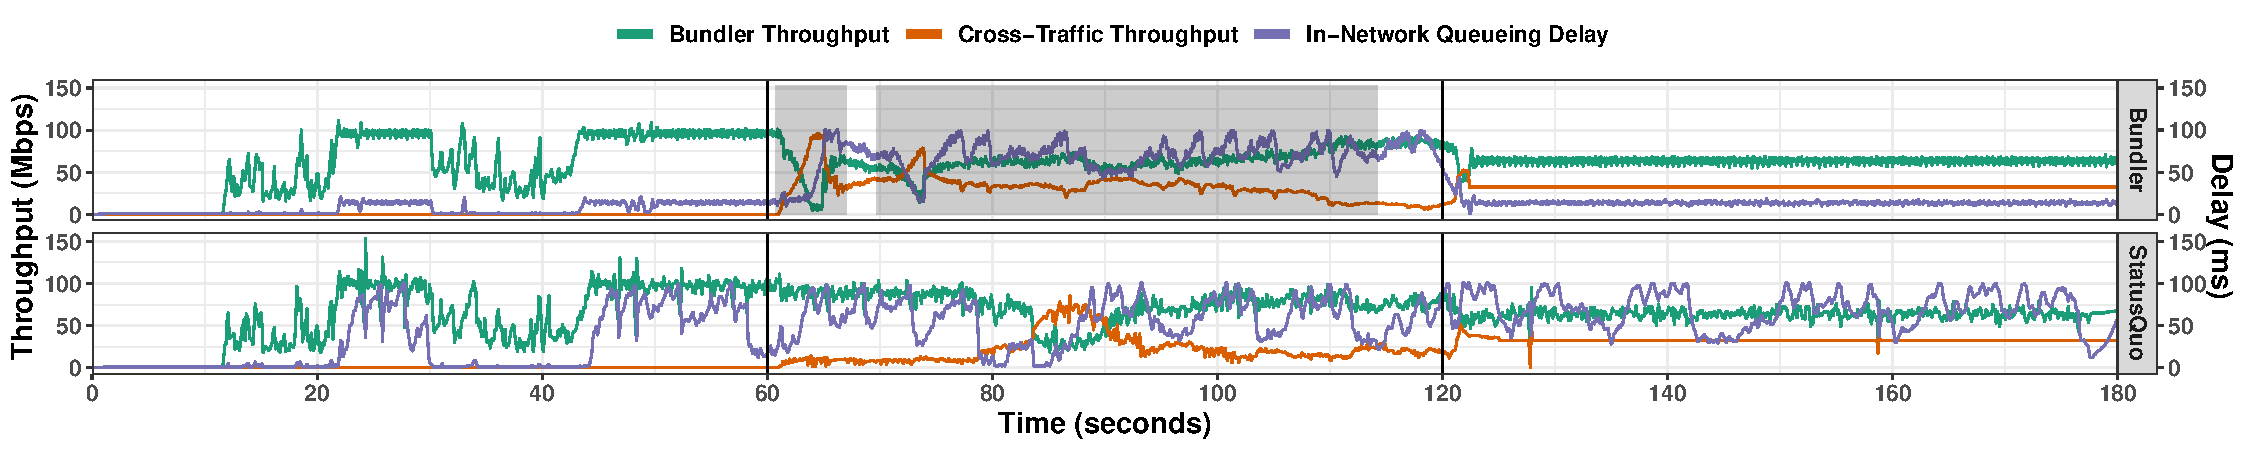
\includegraphics[width=\textwidth]{big_exp/timeseries}
\end{centering}
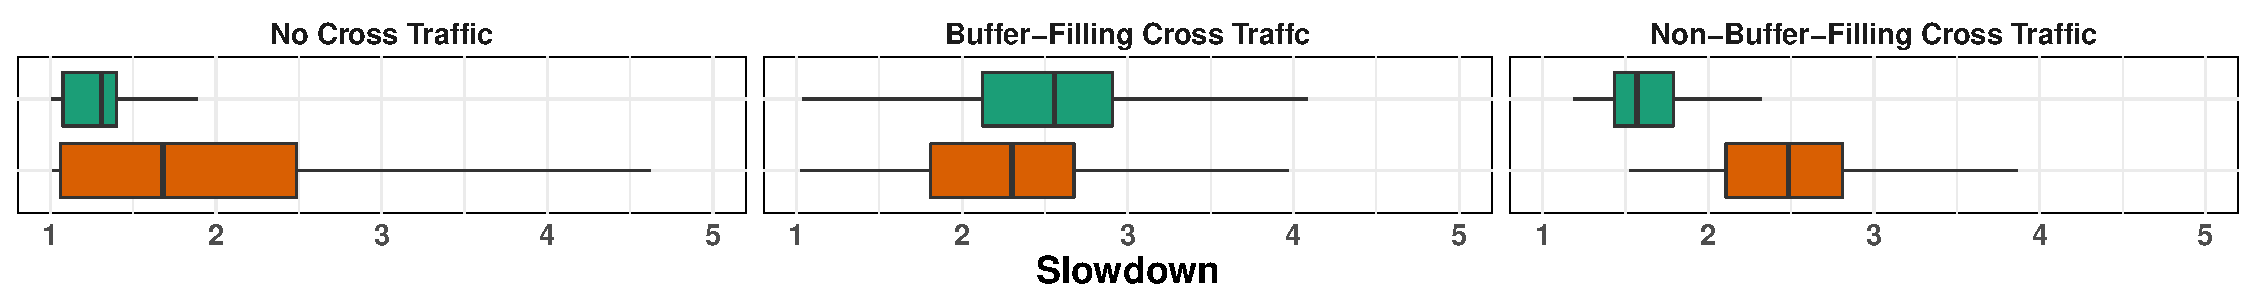
\includegraphics[width=0.95\textwidth]{big_exp/fcts}
\caption{\name's scheduling ability depends on the characteristics of the cross traffic over time. In this experiment, there are 3 periods: from 0 to 60 sec., there is no competing traffic, from 60 to 120 sec. there is buffer-filling cross traffic, and from 120 to 180 sec. there is non-buffer-filling cross traffic. The box-plots below each period show the distribution of short flow FCTs during that time. During the period with buffer-filling cross traffic, \name detects its presence and competes fairly. The shaded region indicates time \name spent in buffer-filling cross-traffic mode (\Sec{s:buffer-filling}).}\label{fig:eval:bigexp}
\end{figure*}

Can \name successfully revert to status-quo performance in the presence of buffer-filling cross traffic, then resume providing benefits once that cross traffic leaves?
In Figure~\ref{fig:eval:bigexp}, we show this scenario.
At first, the link is occupied only by \name's traffic, similar to the setup described in \S\ref{s:eval:setup}.
At time $t=60$~sec, a buffer-filling cross traffic flow arrives.
\name detects its presence (indicated by the gray shading) and starts pushing more packets into the network to compete fairly, reverting back to performance that is slightly worse than Status Quo (median FCT for short flows is \bigexpElasticSlowdownWorseness higher). 
Performance is slightly worse because of the $10$ms queue that \name continues to maintain at its \inbox for active probing to detect the cross-traffic's departure, as described in \S\ref{s:queue-ctl}.
\footnote{We believe the benefits provided by \name in the more common regime with no competing buffer-filling cross traffic are substantial enough to make up for slight degradation in these specific scenarios.}
At time $t=120$sec, the buffer-filling flow stops and non-buffer-filling traffic starts, generated from the same distribution as \name as described in \S\ref{s:eval:setup}.
\name correctly detects that it is safe to resume delay-control, and continues providing scheduling benefits.
For the remainder of this subsection, we present three micro-benchmarks which dig deeper into the latter two scenarios, where cross traffic can affect \name's performance. 
We present results with both Nimbus and Copa being used as the congestion control algorithm at the \inbox. 
\cut{In \S\ref{s:eval:offeredload} we present further results on how well \name retains benefits with varying amounts of offered load.}

\begin{figure}
    \centering
\begin{knitrout}
\definecolor{shadecolor}{rgb}{0.969, 0.969, 0.969}\color{fgcolor}
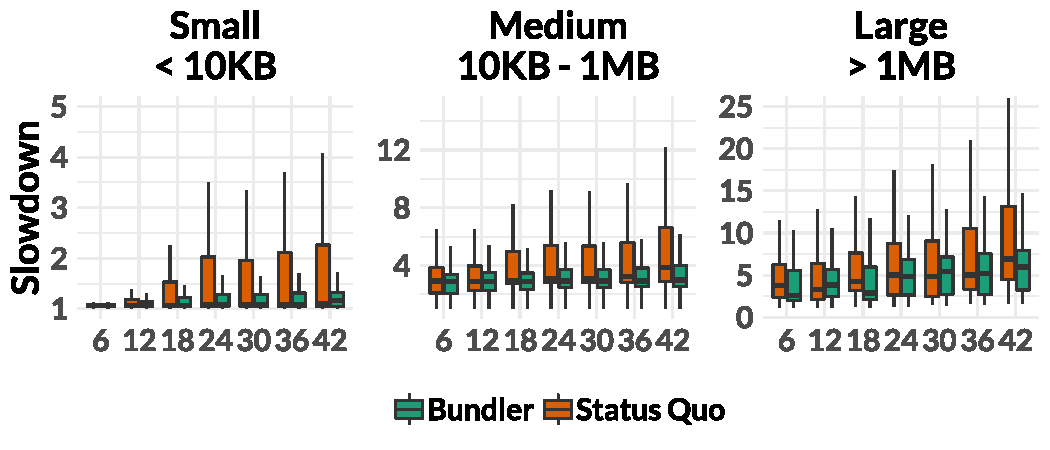
\includegraphics[width=\maxwidth]{figure/robust_cr-inelastic-1} 

\end{knitrout}
    \caption{Against cross traffic comprising of short lived flows. \name offers 48Mbps of load to the bottleneck queue. The cross traffic's offered load increases along the x-axis, while \name{}'s offered load remains fixed.}
    \label{fig:robust:cr-inelastic}
\end{figure}

\paragrapha{Mix of flow sizes} 
We first consider in Figure~\ref{fig:robust:cr-inelastic} the case \name traffic is most likely to encounter, where the cross traffic comprises of finite-length flows up to a few MBs.
We draw both \name's traffic and the cross traffic from the same measured distribution of web requests described in \S\ref{s:eval:setup}.
We fix \name's offered load at a constant $48$ Mbit/s and vary the cross traffic's offered load from $6$ to $42$ Mbit/s.

While flows are often short, they sometimes exit slow start. With sufficient offered load, they can cause queueing in the aggregate. 
Observe that the \baseline FCTs increase steadily as the cross traffic's offered load increases: this is due to the aggregate queueing effect.
When this happens, Bundler responds by temporarily reducing its sending rate to lower the delay, because the cross traffic has not been deemed elastic. 
Importantly, this rate reduction is short-lived because these cross-traffic flows are short-lived, and long-term Bundler throughput is not reduced.
We believe that this trade-off (short-term throughput reduction for better delay) is a good one. 
The lower delay helps the short flows in the bundle, while the large flows in the bundle are not affected by the short-term throughput reduction. 
``Mid-sized'' flows in the bundle can be affected if \name sacrifices throughput for too long. 
By design, however, \name detects such cross-traffic and disables its delay-control mechanism in response.

\begin{figure}
    \centering
    \begin{subfigure}[b]{0.5\textwidth}
\begin{knitrout}
\definecolor{shadecolor}{rgb}{0.969, 0.969, 0.969}\color{fgcolor}
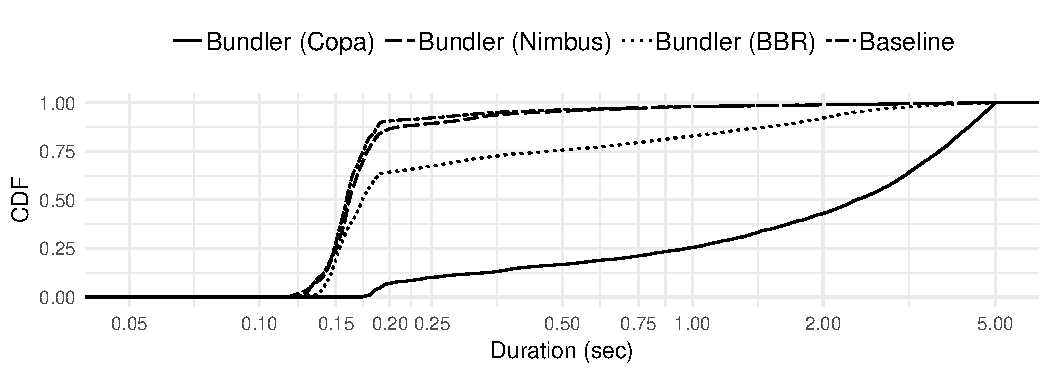
\includegraphics[width=\maxwidth]{figure/robust:cr-elastic:a-1} 

\end{knitrout}
    \caption{Congestion controllers from \S\ref{s:eval}.}\label{fig:robust:cr-elastic:a}
    \end{subfigure}
    \begin{subfigure}[b]{0.5\textwidth}
\begin{knitrout}
\definecolor{shadecolor}{rgb}{0.969, 0.969, 0.969}\color{fgcolor}
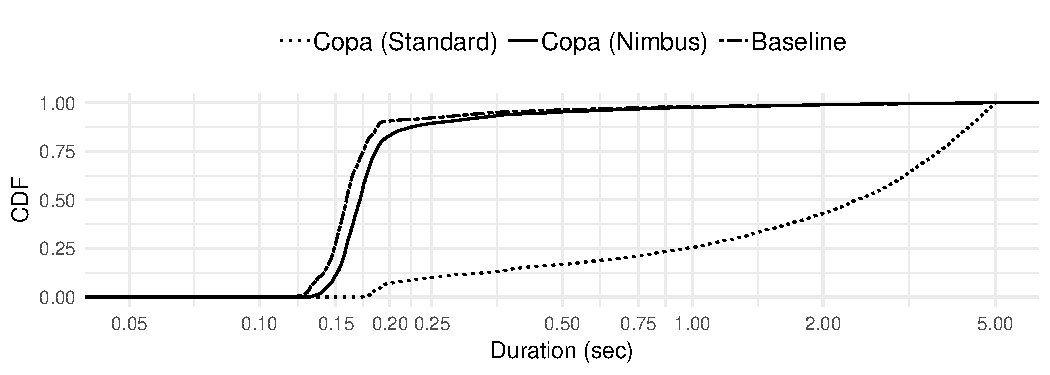
\includegraphics[width=\maxwidth]{figure/robust:cr-elastic:b-1} 

\end{knitrout}
    \caption{Alternate configuration -- Copa uses Nimbus's elasticity detector.}\label{fig:robust:cr-elastic:b}
    \end{subfigure}

    \caption{Elastic cross traffic.}
    \label{fig:robust:cr-elastic}
\end{figure}

\paragrapha{Persistent elastic flows} 
We now evaluate how \name's throughput is impacted due to competition from varying amounts of persistent elastic cross-traffic. 
As discussed in \S\ref{s:queue-ctl}, we believe this synthetic scenario is rare in practice, but when it does occur, \name cannot provide benefits, and since it must ``hold back'' some queue to detect when the cross-traffic subsides, its traffic will experience RTT inflation.
Indeed, Figure~\ref{fig:robust:cr-elastic} shows that 
the component flows in the bundle experience  \bundlerElasticTputWorseness less throughput on average. 
The impact varies from \bundlerElasticTputWorsenessTen lower throughput with 10 competing flows to \bundlerElasticTputWorsenessFifty lower with 50. 

\begin{figure}
    \centering
\begin{knitrout}
\definecolor{shadecolor}{rgb}{0.969, 0.969, 0.969}\color{fgcolor}
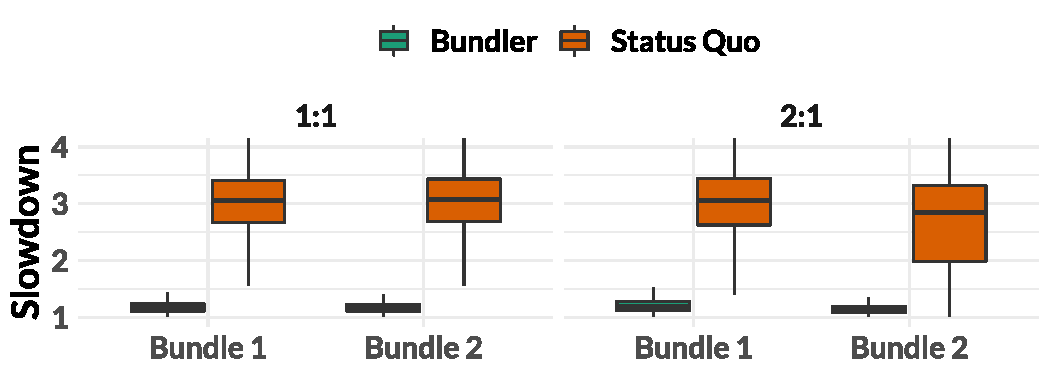
\includegraphics[width=\maxwidth]{figure/robust_twobundler-1} 

\end{knitrout}
    \caption{Competing traffic bundles. In both cases, the aggregate offered load is 84Mbps, as in Figure~\ref{fig:eval:best}. For "1:1", we evenly split the offered load between the two Bundles; for "2:1", one bundle has twice the offered load of the other. In both cases, each bundle observes improved median FCT compared to its performance in the baseline scenario.}
    \label{fig:robust:twobundler}
\end{figure}

\paragrapha{Competing Bundles} Last, we evaluate the case where flows from multiple bundles compete with one another. 
In Figure~\ref{fig:robust:twobundler}, we show the performance with two bundles of traffic competing with one another at the same bottleneck link. 
Both bundles comprise of web requests along with a backlogged Cubic flow. 
%Even in the presence of this buffer-filling cross traffic, 
%\radhika{??? i believe the backlog flow is in the bundles and not outside it}
%\an{yes, it is, that's why the perf is good. I agree we should reword, it is confusing}
Both bundles maintain low queueing in the network and successfully control the queues at the \inbox.
Thus, \name provides benefits for both bundles, even when the amount of traffic in each bundle is different.  

\subsection{Impact of Congestion Control}\label{s:eval:cc}

%\an{I have cut down this subsection: removed the e2e congestion control figure and replaced with inline text}
We now evaluate the impact of a different congestion control algorithm running at the \inbox and at the endhosts.

\begin{figure}
    \centering
\begin{knitrout}
\definecolor{shadecolor}{rgb}{0.969, 0.969, 0.969}\color{fgcolor}
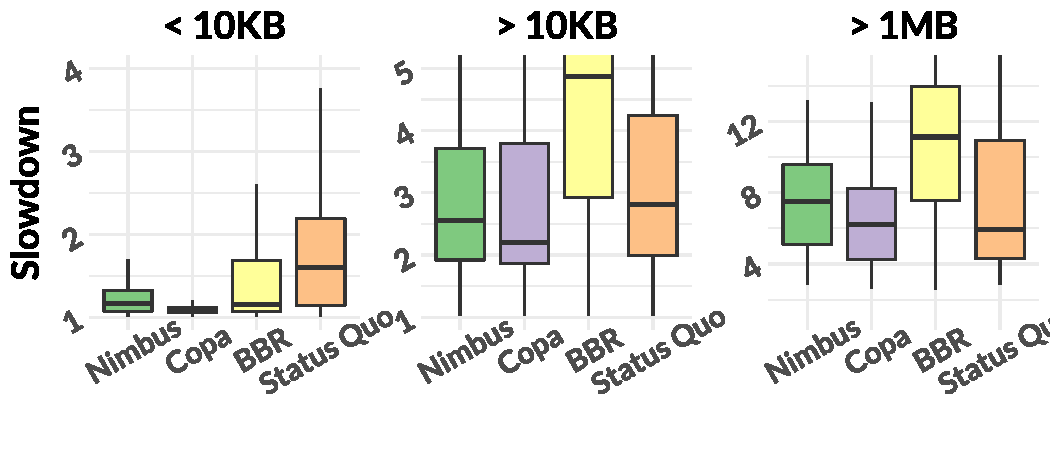
\includegraphics[width=\maxwidth]{figure/eval:cc-1} 

\end{knitrout}
    \caption{Choosing a congestion control algorithm at \name remains important, just as it is at the end-host. Note the different y-axis scales for each group of request sizes.}
    \label{fig:eval:cc}
\end{figure}
\newcommand{\ccCopaMedian}{}
\newcommand{\ccNimbusMedian}{}
\newcommand{\ccBBRMedian}{}
\newcommand{\ccBaselineMedian}{}


\Para{\capinbox congestion control} So far we have evaluated \name by running Copa~\cite{copa} at the \inbox. 
Figure~\ref{fig:eval:cc} shows \name's performance with other congestion control algorithms (namely, Nimbus's BasicDelay~\cite{nimbus-arxiv} and BBR~\cite{bbr}), and using SFQ scheduling. 
We find that using BasicDelay provides similar benefits over \baseline as Copa. 
BBR, on the other hand, performs slightly worse than \baseline. 
This is because it pushes packets into the network more aggressively than the other schemes, resulting in a bigger in-network queue.
This, combined with the queue built at the \name, results in the endhosts experiencing higher queueing delays than \baseline. This shows that the choice of congestion control algorithm, and its ability to maintain small queues in the network, plays an important role. 

\Para{Endhost congestion control} We used Cubic congestion control at the endhosts for our experiments so far. When we configure endhosts to use Reno or BBR, \name's benefits remain: \name achieves 58\% lower FCTs in the median compared to the updated \baseline where the endhosts use BBR. 
This shows that \name is compatible with multiple endhost congestion control algorithms.
%This is primarily because in the \baseline, using BBR causes endhosts to achieve 66\% worse median slowdown ($1.62$ with Cubic to $2.68$ with BBR); \name's slowdown is only 5\% worse when endhosts use BBR ($1.08$ with Cubic to $1.14$ with BBR). 

\cut{
\begin{figure}
    \centering
\begin{knitrout}
\definecolor{shadecolor}{rgb}{0.969, 0.969, 0.969}\color{fgcolor}
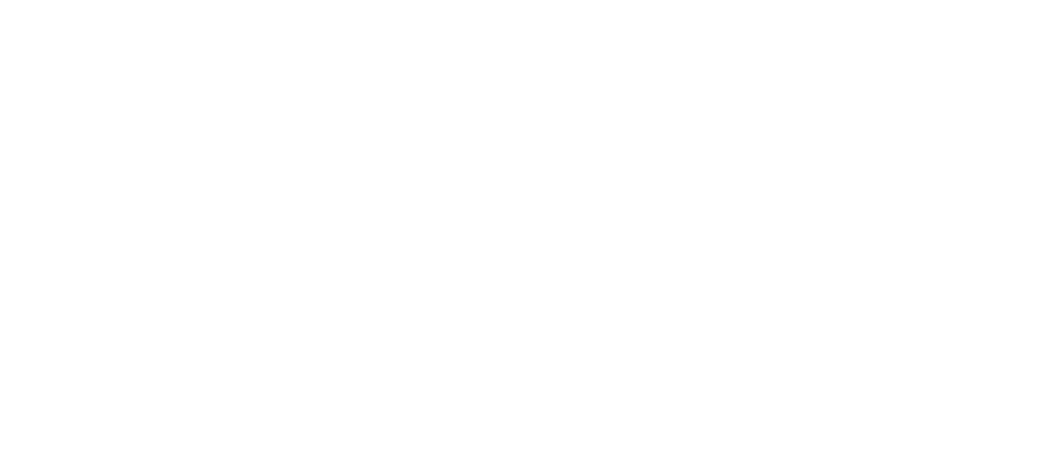
\includegraphics[width=\maxwidth]{figure/eval_e2e-1} 

\end{knitrout}
    \caption{\name still provides benefits when the endhosts use different congestion control algorithms.}
    \label{fig:eval:traffic}
\end{figure}

\Para{Endhost congestion control} 
We used Cubic congestion control at the endhosts for our experiments so far. When we configure endhosts to use Reno or BBR (as implemented in Linux $4.13$), \name's benefits remain (Figure~\ref{fig:eval:traffic}).
%: in Figure~\ref{fig:eval:traffic}, \name achieves 58\% lower FCTs in the median compared to the updated \baseline where the endhosts use BBR. 
%This is primarily because in the \baseline using BBR causes endhosts to achieve 66\% worse median slowdown ($1.62$ with Cubic to $2.68$ with BBR); \name's slowdown is only 5\% worse when endhosts use BBR ($1.08$ with Cubic to $1.14$ with BBR). 
This shows that \name is compatible with multiple endhost congestion control algorithms.
}


\subsection{Varying Offered Load}\label{s:eval:offeredload}
%Naturally, if a link is less congested, scheduling the packets that traverse it will have less benefit. Accordingly, as the offered load is reduced, we would expect the gains from scheduling to diminish. 
We now use the web request distribution described in \S\ref{s:eval:setup} to generate a load of 50\% ($48$Mbps), 75\% ($72$Mbps) and 87.5\% ($84$Mbps) of the bottleneck link bandwidth. Our results in Figure~\ref{fig:eval:offeredload} show that as the offered load is decreased, the benefits of \name reduce. This is because if a link is less congested, scheduling the packets that traverse it will have less benefit.
% At 87.5\% load, even without the load offered by a persistently backlogged connection, \name improves FCTs by \an{amount}. 
% As the offered load decreases to 50\%, the benefit provided by \name decreases as well -- to \an{amount} at the 75th percentile.

\begin{figure*}[ht!]
    \centering
\begin{knitrout}
\definecolor{shadecolor}{rgb}{0.969, 0.969, 0.969}\color{fgcolor}
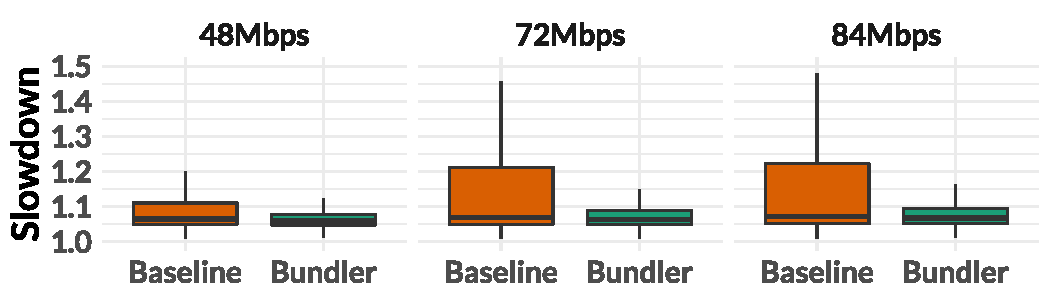
\includegraphics[width=\maxwidth]{figure/eval:offeredload-1} 

\end{knitrout}
    \caption{\name offers diminishing returns with lower amounts of offered load.}
    \label{fig:eval:offeredload}
\end{figure*}
%
%\newcommand{\highUtilTailImprove}{round(highUtilTailImprove, 0)\%\xspace}
%\newcommand{\medUtilTailImprove}{round(medUtilTailImprove, 0)\%\xspace}
%\newcommand{\lowUtilTailImprove}{round(lowUtilTailImprove, 0)\%\xspace}


\subsection{Terminating TCP Connections}\label{s:eval:proxy}

We now study the benefits of combining \name with a TCP proxy middlebox. A TCP-proxy enables the the end-to-end congestion controller to observe a smaller RTT, by acknowledging its segments much faster than the original receiver further away. This enables a rapid window growth at the endhosts, causing packets to arrive at a faster rate at the middlebox. Combining \name with such a proxy would result in even greater scheduling opportunities. 

To evaluate this, we emulate a TCP proxy by modifying the endhosts to maintain a constant congestion window of $450$ packets---slightly larger than the bandwidth-delay product in our setup---and increase the buffering at the \inbox to hold these packets. The other aspects of \name remain unchanged, including its use of Copa to move the queues from the network, and its proper scheduling.
The result is in Figure~\ref{fig:eval:proxy}. As expected, combining \name with a TCP proxy produces even greater benefits, though primarily for large flows that benefit from the increased congestion window. 
%For the short requests which never leave TCP slow start, terminating TCP connections does not yield additional benefits: with or without termination, they finish in a few RTTs.
%A proxy-based design could then apply a scheduling policy to the acknowledged, but yet unsent traffic from terminated connections.



% An alternate implementation of a \name could terminate TCP connections at the \inbox. 
% %\radhika{I assume we mention this in an earlier section? else we need a line or two about why this experiment is interesting.}
% We consider the best-case outcome of terminating TCP connections --- the RTT the end-to-end congestion controller observed would decrease (since the proxy would acknowledge its segments much faster than the original receiver would), and it would therefore grow its window rapidly.
% A proxy-based design could then apply a scheduling policy to the acknowledged, but yet unsent traffic from terminated connections.
% To emulate a best-case scenario for termination, we modify the end-hosts to maintain a constant congestion window of $450$ packets --- slightly larger than the BDP --- and increase the buffering at the \inbox to hold these packets. 
% The other aspects of \name, including scheduling, remain unchanged.
% The result is in Figure~\ref{fig:eval:proxy}.
%
\begin{figure}
    \centering
\begin{knitrout}
\definecolor{shadecolor}{rgb}{0.969, 0.969, 0.969}\color{fgcolor}
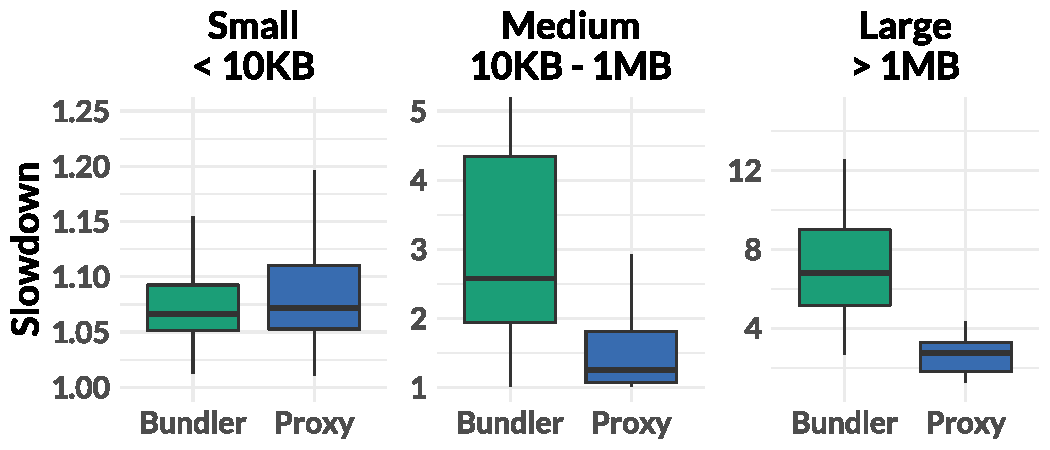
\includegraphics[width=\maxwidth]{figure/eval_proxy-1} 

\end{knitrout}
    \caption{A proxy-based implementation of \name could yield further benefits to the long flows. Note the different y-axis scales for each group of request sizes.}
    \label{fig:eval:proxy}
\end{figure}

%
%For the short requests which never leave TCP slow start, terminating TCP connections does not yield additional benefits: with or without termination, they finish in a few RTTs.
%For medium-to-long requests, terminating TCP connections yields benefits since they no longer incur the penalty of window growth.
